\chapter{Fundamentação Teórica}

Neste capítulo será introduzido alguns conceitos essenciais para ajudar no entendimento
da proposta desse trabalho. Entre eles, LPWAN, a tecnologia LoRa e Protocolos de Controle
de Acesso ao Meio.

\section{Low Power Wide Area Network}

Low Power Wide Area Network ou LPWAN são tecnologias de rede sem fio que proporcionam comunicação
entre dispositivos a longas distancias com um baixo custo energético. A principal motivação para
o desenvolvimento das LPWAN é a Internet das Coisas, uma vez que as tecnologias de rede tradicionais
não foram desenvolvidas para o cenário atual IoT. As principais vantagens das LPWAN quando comparadas
com as outras redes são: seu alcance quilométrico, alta autonomia de bateria, e suporte para vários
dispositivos na rede. A maior desvantagem é a baixa largura de banda, como pode ser visto na imagem
\ref{fig:lpwan} a seguir. Apesar da baixa largura de banda, LPWAN continua sendo uma ótima opção
para maioria das soluções IoT que no geral não transmitem dados de grande volume. \cite{9243410}

\begin{figure}[H]
    \centering
	\caption{Comparativo entras as tecnologias de redes: Largura de Banda versus Distância}
    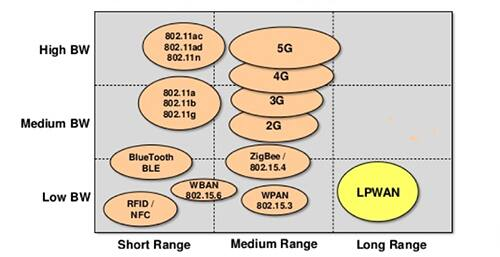
\includegraphics[width=0.9\textwidth]{img/lpwan.jpg}
    \label{fig:lpwan}
    
    Fonte: Link Labs, Peter R. Egli, 2015.
\end{figure}

\subsection{Tecnologias LPWAN existentes}

Atualmente existem diversas tecnologias LPWAN e elas podem ser divididas em duas categorias: espectro
aberto, e espectro licenciado. Isso significa que algumas tecnologias LPWAN operam numa faixa de frequência que é necessário pagar para o uso, e outras usam a faixa de frequência livre de diversos
países, porem isso implica em determinados países algumas regras de uso e também o compartilhamento
da faixa com outros dispositivos. Dentre as tecnologias mais famosas podem ser destacadas a NB-IoT,
Sigfox e LoRa, presentes em diversas soluções IoT de longas distâncias. Na figura \ref{fig:lpwans}
a seguir é possível visualizar algumas das tecnologias LPWAN. \cite{fi12030046}

\begin{figure}[H]
    \centering
	\caption{Tecnologias LWPAN}
    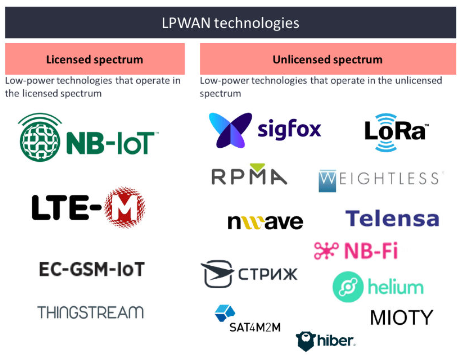
\includegraphics[width=0.7\textwidth]{img/lpwans.png}
    \label{fig:lpwans}
    
    Fonte: IoT Analytics LPWAN Mark Report 2018 - 2023, Romeo, 2019.
\end{figure}

\section{LoRa}

LoRa é uma tecnologia LPWAN que significa Long Range, foi criada em 2008 pela Cycleo SAS e adquerida
em 2012 pela Semtech, e é atualmente mantida pela LoRa Alliance. LoRa usa bandas de radiofrequência
sub-gigahertz de livre uso que podem variar entre 433 MHz, 868 MHz, 915 MHz e 923 MHz dependendo do
país. A tecnologia LoRa implementa uma camada física de comunicação, deixando aberto assim para outras
tecnologias cobrirem a responsabilidade das camadas acima, a mais conhecida para isso atualmente é a LoRaWAN, um protocolo de controle de acesso ao meio também mantido pela LoRa Alliance.  \cite{8474715}

\newpage

\subsection{Modulação LoRa}

A modulação LoRa é proprietária da Semtech e baseada em CSS, do inglês Chirp Spread Spectrum.
Diferente de modulações mais convencionas como FSK (Frequency-shift keying) que codifica
os símbolos para frequências especificas, a modulação LoRa codifica seus símbolos baseando-se no
incremento linear da frequência, gerando o que é chamado de "chirp". Na figura \ref{fig:lora1}
a seguir é possível ver esse "chirp" no domínio da franquênia e como é o sinal no domínio do
tempo. \cite{8067462}

\begin{figure}[H]
    \centering
	\caption{Chirp Spread Spectrum: Domínio da Franquênia e Domínio do Tempo}
    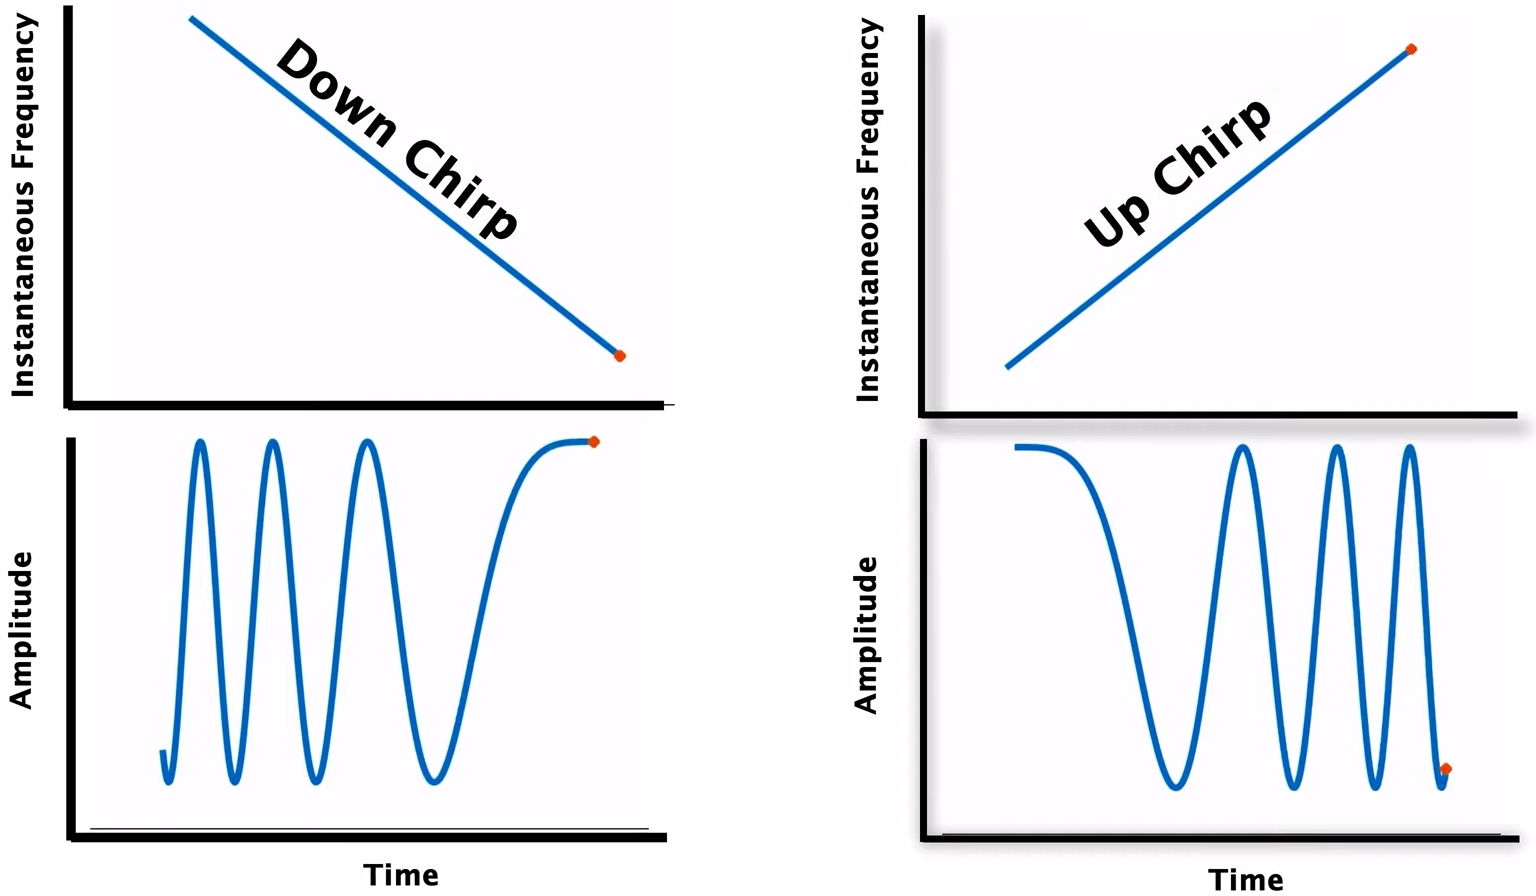
\includegraphics[width=0.7\textwidth]{img/lora1.png}
    \label{fig:lora1}
    
    Fonte: Visual Electric Youtube Channel, 2021.
\end{figure}

Na figura \ref{fig:lora2} a seguir, podemos ver uma representação matemática de uma sinal na modulação LoRa,
apesar de relativamente complexa, podemos analisa-lá de uma maneira mais simplória para entender como
a Tecnologia LoRa gera diferentes "chirps" para codificar os símbolos.

\begin{figure}[H]
    \centering
	\caption{Representação matemática de um sinal LoRa}
    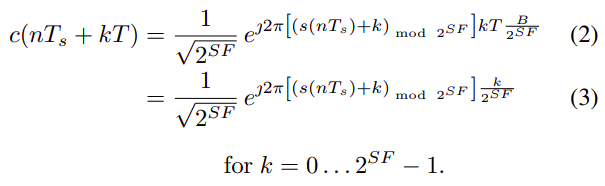
\includegraphics[width=0.8\textwidth]{img/lora2.png}
    \label{fig:lora2}
    
    Fonte: Frequency Shift Chirp Modulation: the LoRa™ Modulation, Lorenzo Vangelista, 2017.
\end{figure}

Focando apenas na exponencial complexa, sabemos pela matemática que isso representa uma onda senoidal,
onde a frequência base é determinada por \(s(nT_{s})\) e gradualmente incrementada por \(k\), e isso por
si só já forma o "chirp" visto na figura \ref{fig:lora1}. O grande truque está no \(\mod 2^{SF}\), esse
módulo garante que a frequência incremente até o limite superior da largura de banda, e volte para o limite
inferior, gerando assim uma descontinuidade no "chirp" que pode ser visto na figura \ref{fig:lora3-4} a
seguir. \cite{8067462}

\begin{figure}[H]
    \centering
        \caption{Modulação LoRa: Descontinuidade e Largura da Banda}
        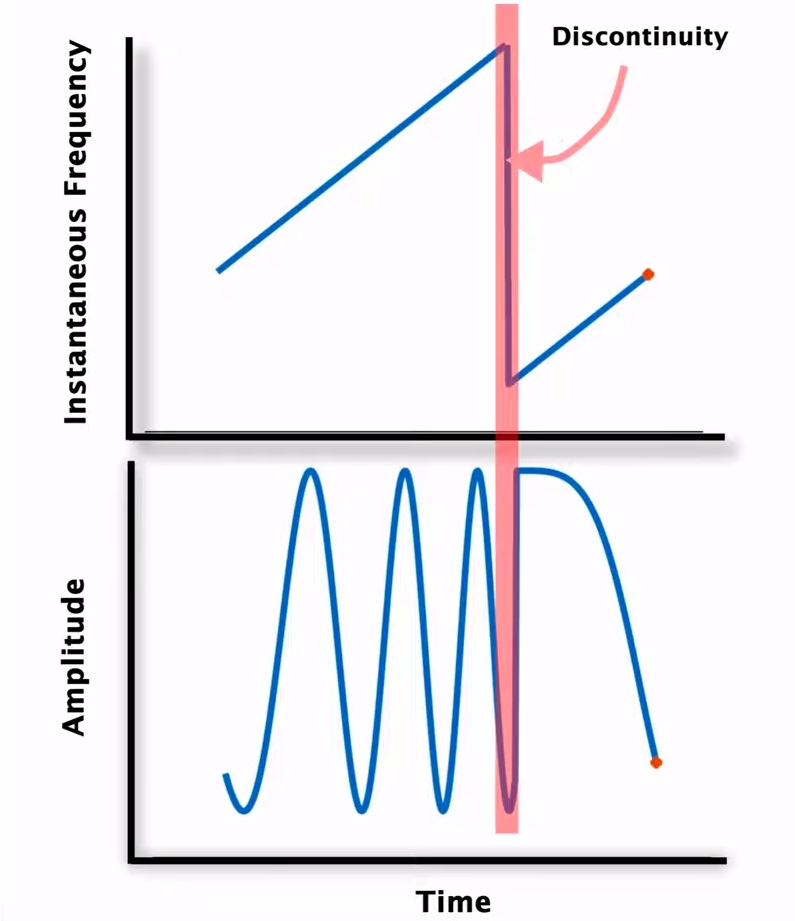
\includegraphics[width=.4\linewidth]{img/lora3.png}
        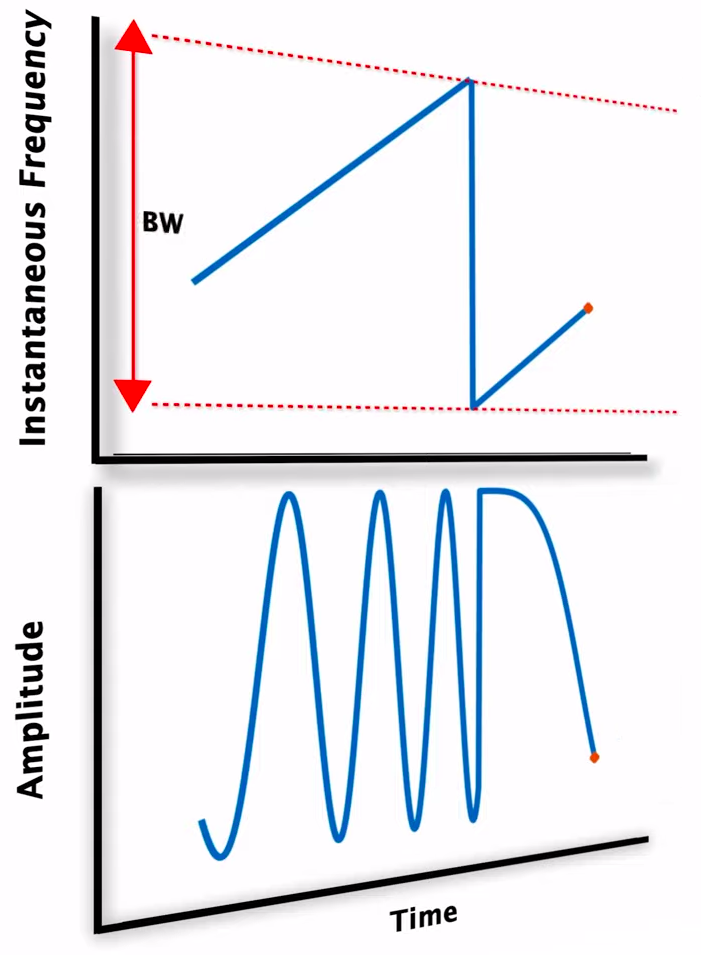
\includegraphics[width=.35\linewidth]{img/lora4.png}
    \label{fig:lora3-4}

    Fonte: Visual Electric Youtube Channel, 2021.
\end{figure}

Dessa forma, a codificação de um símbolo na modulação LoRa se encontra em qual momento dentro da
duração de um sinal ocorre essa descontinuidade. Na figura \ref{fig:lora5} seguir podemos ver
alguns exemplos de sinais LoRa com diferentes momentos de descontinuidade.

\begin{figure}[H]
    \centering
	\caption{Exemplos de Símbolos LoRa}
    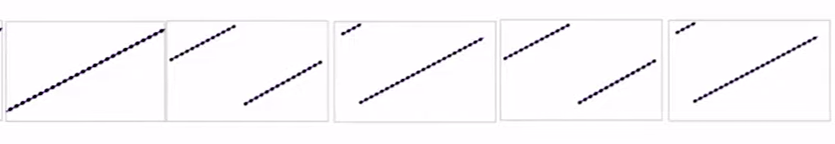
\includegraphics[width=0.8\textwidth]{img/lora5.png}
    \label{fig:lora5}
    
    Fonte: Visual Electric Youtube Channel, 2021.
\end{figure}

Esse tipo de modulação tem suas vantagens e desvantagens, a principal vantagem é robustez do sinal
a longas distâncias, e a principal desvantagem é que, por toda largura de banda ser usada para a codificação de cada símbolo, isso implica numa taxa da envio de dados mais baixa quando comparado
a outras modulações.

Uma característica importante na modulação LoRa é o termo SF visto na função do módulo, ele significa
"Spreading Factor" e representa um numero inteiro que pode ser de 7 a 12. o Spreading Factor determina
duas coisas importantes: a duração de um símbolo, e a quantidade possíveis de símbolos que podem ser
codificados. Quanto maior o Spreading Factor maior é o tempo para enviar um símbolo e maior também é
a quantidade símbolos. Na figura \ref{fig:lora6} a seguir podemos ver uma comparação entre os Spreading
Factors. \cite{8067462}

\newpage

\begin{figure}[H]
    \centering
	\caption{LoRa Spreading Factor}
    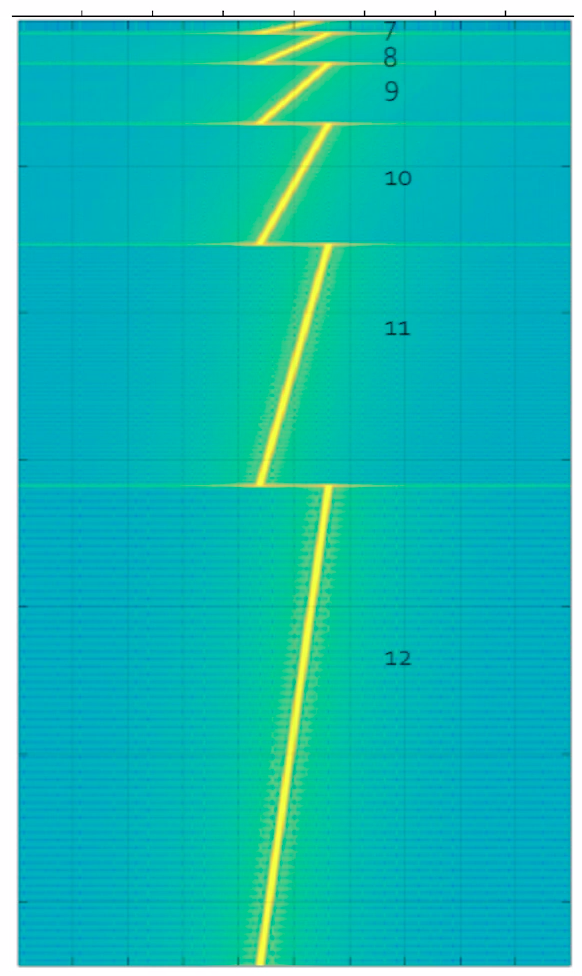
\includegraphics[width=0.32\textwidth]{img/lora6.png}
    \label{fig:lora6}
    
    Fonte: Richard Wenner Youtube Channel, 2017.
\end{figure}

Outra característica influenciada pelo Spreading Factor é a taxa de envio de dados, que diminui a
medida que o SF aumenta, pelo simples fato de que o envio de cada símbolo dura mais tempo, mas também
se aumenta a robustez do sinal.

Como o momento em que a descontinuidade ocorre no "chirp" é um ponto essencial para a decodificação,
o receptor precisa de certa forma saber identificar quando é o começo e o final de um sinal. Para isso
existe o que é chamado de "Preamble", que é um conjunto de sinais idênticos que são enviados uma quantidade fixa de vezes antes de qualquer dado significativo, funcionando assim como um tipo de sincronização. Na figura \ref{fig:lora7} a seguir é possível ver uma exemplo. \cite{8067462}

\begin{figure}[H]
    \centering
	\caption{LoRa Preamble}
    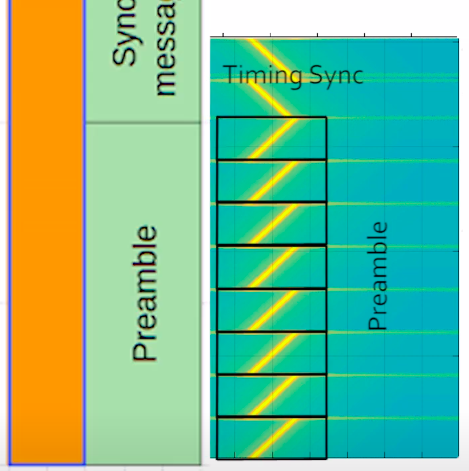
\includegraphics[width=0.34\textwidth]{img/lora7.png}
    \label{fig:lora7}
    
    Fonte: Richard Wenner Youtube Channel, 2017.
\end{figure}

\newpage

Na figura \ref{fig:lora8-9} a seguir é possível ver a estrutura de um Frame LoRa e um exemplo
de um frame no domínio da frequência.

\begin{figure}[H]
    \centering
	\caption{LoRa Frame}
    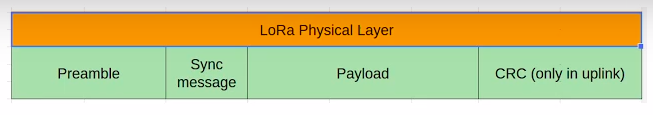
\includegraphics[width=0.8\textwidth]{img/lora8.png}

    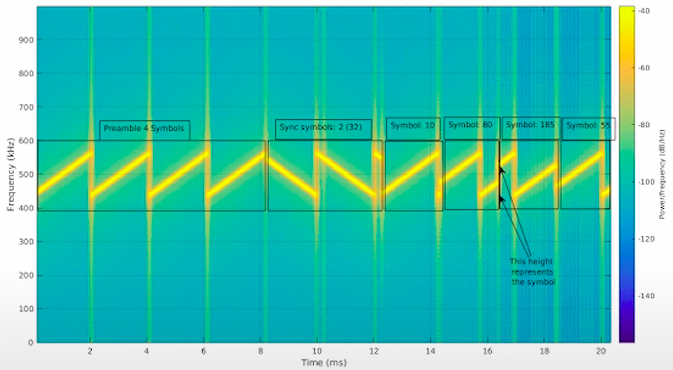
\includegraphics[width=0.8\textwidth]{img/lora9.png}
    \label{fig:lora8-9}
    
    Fonte: Richard Wenner Youtube Channel, 2017.
\end{figure}

\newpage

\section{Protocolos de Controle de Acesso ao Meio}

Protocolos de Controle de Acesso ao Meio, ou do inglês Medium Access Control (MAC), são
protocolos responsáveis por administrar o funcionamento dos hardwares que compõem a camada
física de transmissão de dados, protocolos MAC fazem parte da segunda camada, a camada de
enlace, do modelo OSI, que pode ser vista na figura \ref{fig:osi} a seguir. \cite{5340799}

\begin{figure}[H]
    \centering
	\caption{Camadas do modelo OSI}
    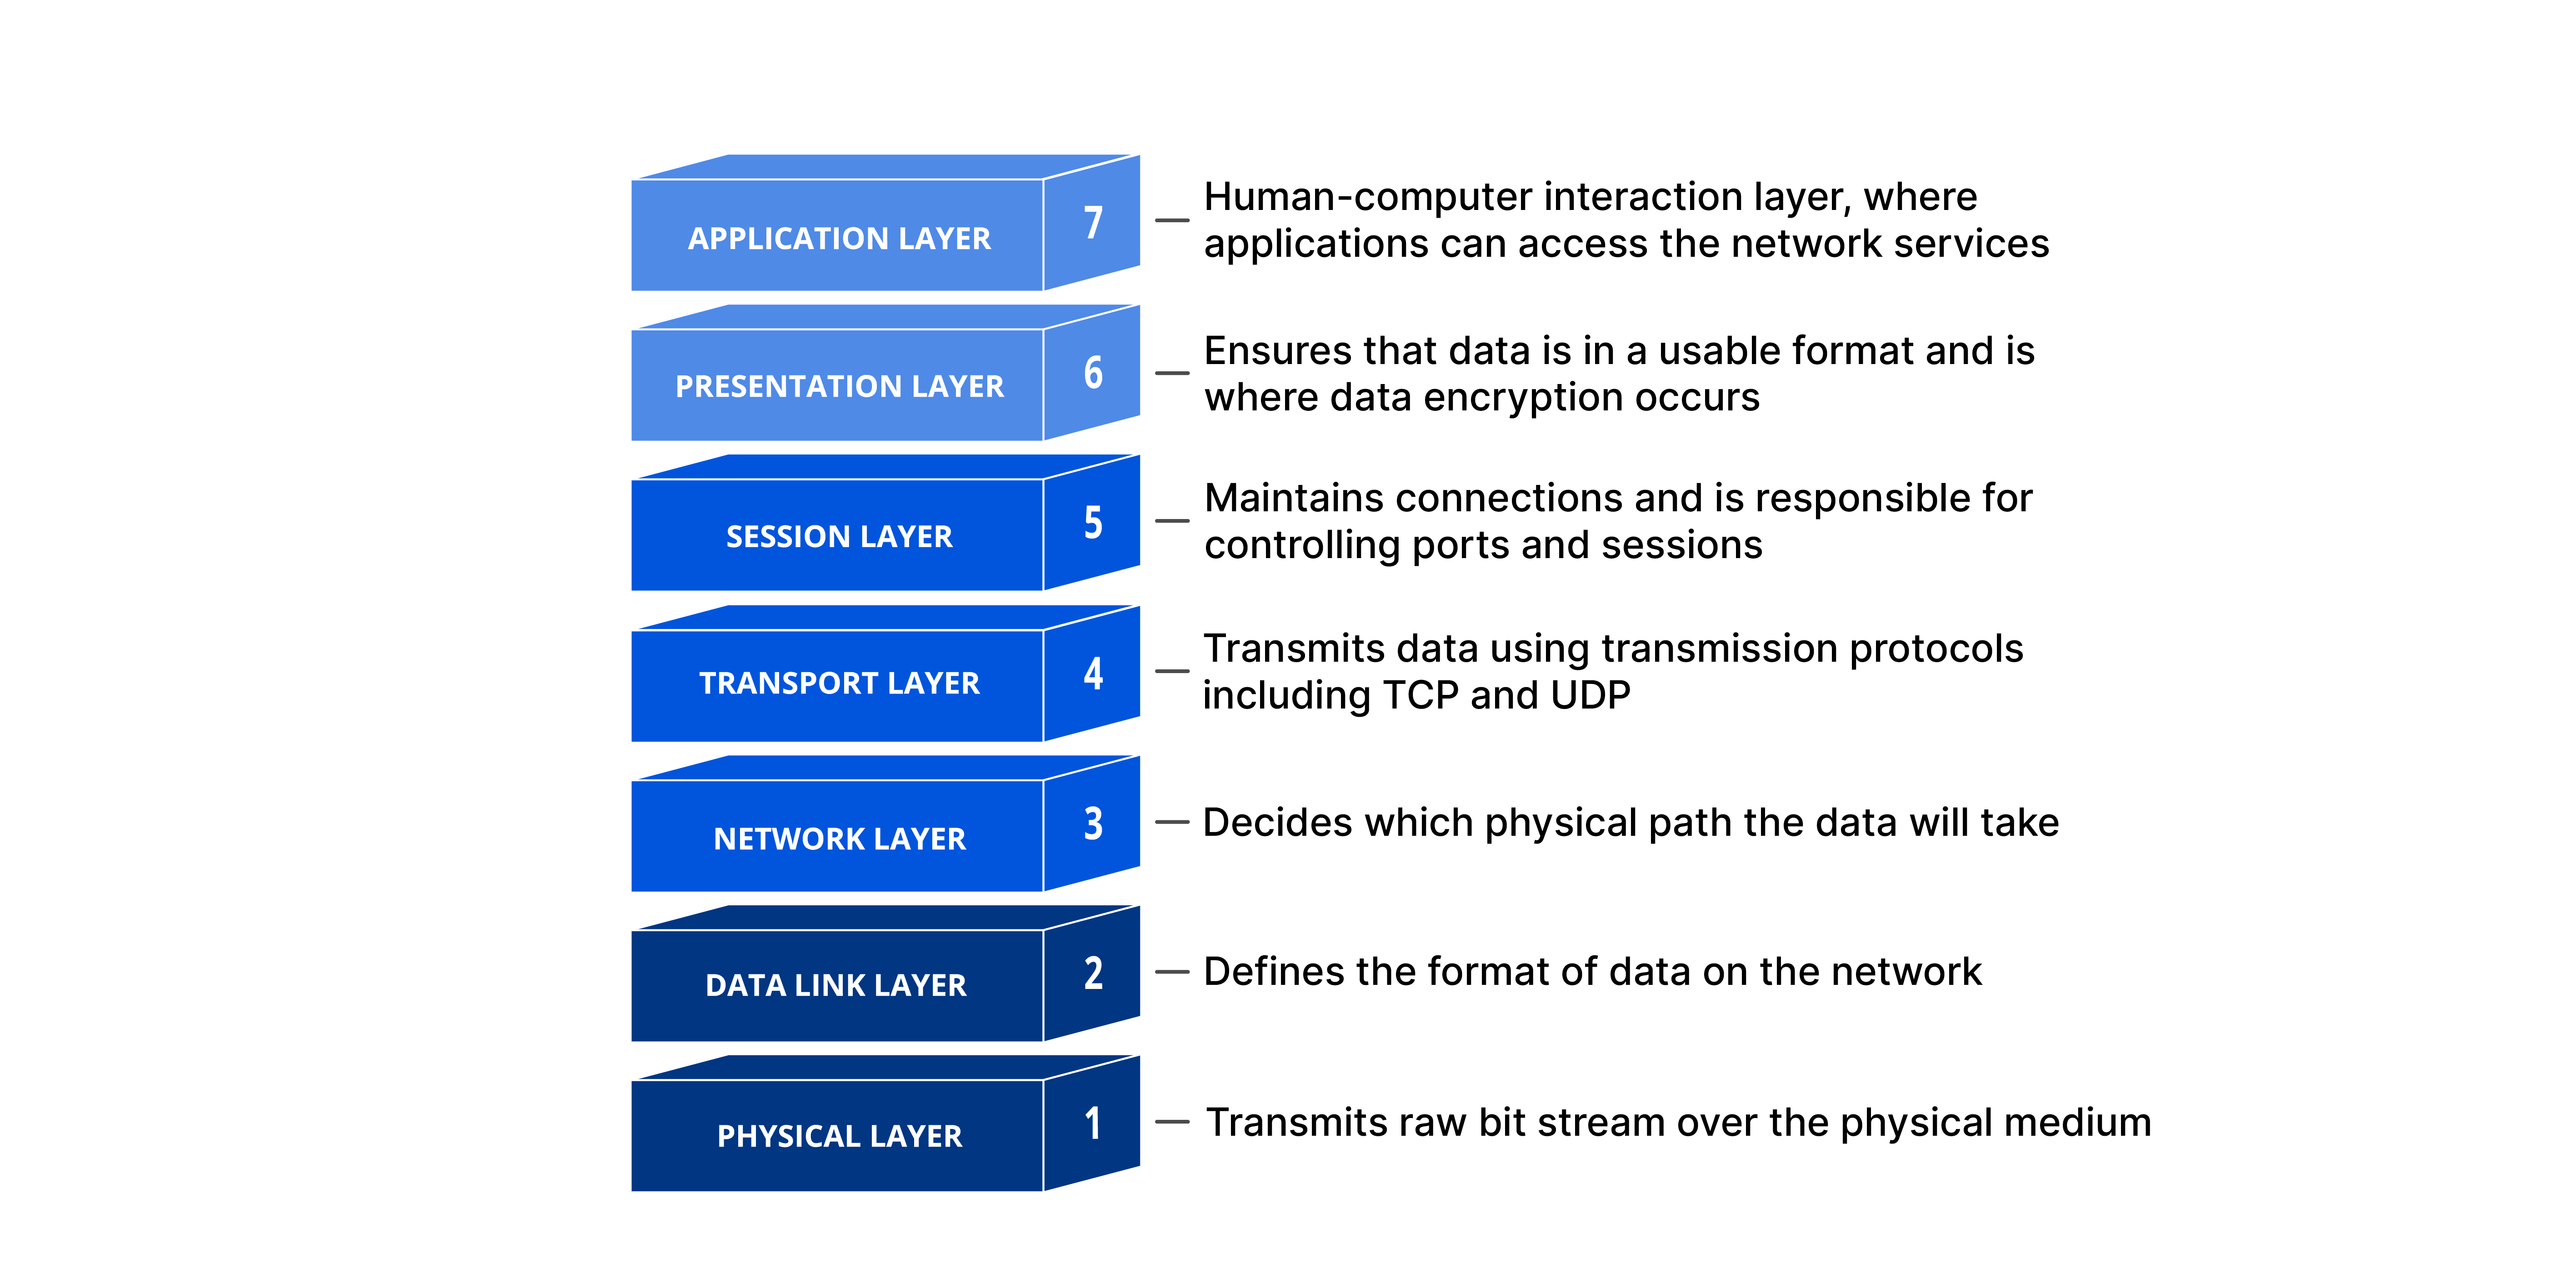
\includegraphics[width=0.9\textwidth]{img/osi-model.png}
    \label{fig:osi}
    
    Fonte: Cloudflare, 2022.
\end{figure}

\subsection{Características de Protocolos MAC}

Protocolos MAC em geral gerenciam o controle de fluxo e a multiplexação de um meio
de comunicação, provendo uma de qualidade de serviço para a camada inferior. Das
características dos protocolos MAC duas mais se destacam: \cite{5340799}

\begin{itemize}
    \item \textbf{Tratamento de Colisão:} Por o canal de comunicação ser normalmente
    compartilhado por outros dispositivos, é normal acontecer colisões, que ocorrem
    quando mais de um dispositivo tentam enviar dados ao mesmo tempo. Cabe ao protocolo
    MAC administrar a vez de uso de cada dispositivo no canal, e também administrar uma
    solução em casos onde pacotes colidem.
    \item \textbf{Detecção de Erros:} Pela natural física de alguns canais de comunicação,
    principalmente os sem fio, é possível que dados que saiam do remetente para o destinatário
    e cheguem corrompidos, assim cabe ao protocolo MAC ter mecanismos de detecção para
    quando esses erros acontecem.
\end{itemize}

\subsection{Exemplos de Algoritmos}

Existem alguns algoritmos conhecidos que garantem as características de um Protocolo MAC,
entre eles temos: \cite{5340799}

\begin{itemize}
    \item \textbf{ALOHA:} O algoritmo ALOHA é um dos mais antigos, surgir na década de 70
    e se destaca pela sua simplicidade: Se você tem dados para mandar, envie-os, Se ocorrer colisão, tente enviar novamente mais tarde. Outra característica desse algoritmo é a divisão
    do dados em pacotes menores que são enviados entre um determinado intervalo de tempo, com isso
    impedia que um único Nó ocupe o canal infinitamente.
    \item \textbf{CSMA/CD:} do inglês Carrier Sense Multiple Access with Collision Detection,
    é um algoritmo mais sofisticado com mecanismo de detecção de colisão. Quando um Nó durante
    a transmissão detecta uma colisão ele imediatamente para a transmissão e enviar um Frame
    de erro, para avisar a todos os nós do canal que houve uma colisão, impedindo que outros
    Nós tentem enviar algum dado. Os Nós que desejam enviar algum pacote deverão esperar um tempo
    aleatório cada para começarem uma nova transmissão.
    \item \textbf{CSMA/CA:} Já o CSMA/CA, do inglês Carrier Sense Multiple Access with Collision Avoidence, utiliza de sinal RTS (Request to Send) e CTS (Clear to Send). Qualquer Nó que
    deseja fazer uma transmissão manda um sinal RTS e só poderá começar o envio após receber
    um CTS, qualquer outro Nó ao perceber esses sinais no canal evitam fazer uma transmissão
    por um determinado período de tempo.
    \item \textbf{Token Ring:} O algoritmo Token Ring foi criado na década de 60 pela IBM e
    apenas funciona em redes com topologia Anel, é uma algoritmo simples onde um token é passado
    de Nó a Nó e apenas quem está com o Token pode transmitir. Se um Nó com o Token não deseja
    transmitir, ele transfere o Token para o próximo Nó, além disso cada Nó pode ficar com o
    Token por um determinado tempo.
\end{itemize}